\section{Second-order nonlinear time-invariant systems}
We first consider the system
\begin{equation}
\begin{array}{l}{\dot{x}_{1}=f_{1}\left(x_{1}, x_{2}\right)} \\ {\dot{x}_{2}=f_{2}\left(x_{1}, x_{2}\right)}\end{array}
\end{equation}

\textbf{Phase-plane analysis:} Determine the system behavior by constructing a \hl{phase portrait}, i.e. plotting different IVP solutions in the phase space.

\begin{tcolorbox}[colback=white, colframe=teal]
\textbf{Local analysis:}
\begin{itemize}[topsep=0pt]
    \item Linearize about $x^*$.
    \item Find eigenvalues $\lambda(A)$.
    \item Classify equilibrium points for $f(x^*) = 0$.
    If $\lambda$ is real, them we either get a stable node ($\lambda_2 < \lambda_1 < 0$), unstable node ($0 < \lambda_2 < \lambda_1$) or a saddle point ($\lambda_2 < 0 < \lambda_1$).
    In the complex case $\lambda_{1,2} = \alpha \pm \beta i$, then we either get a center focus ($\alpha = 0$), a stable focus ($\alpha < 0$) or an unstable focus ($\alpha > 0$).
\end{itemize}
\end{tcolorbox}

\begin{figure}[!htb]
    \centering
    \begin{subfigure}{0.3\textwidth}
        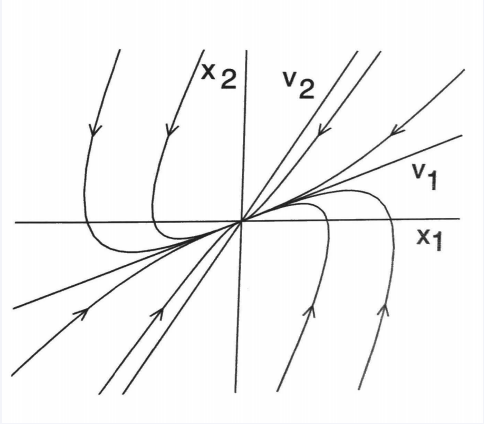
\includegraphics[height=3cm]{figures/sn.png}
        \caption{Stable node}
    \end{subfigure}
    \begin{subfigure}{0.3\textwidth}
        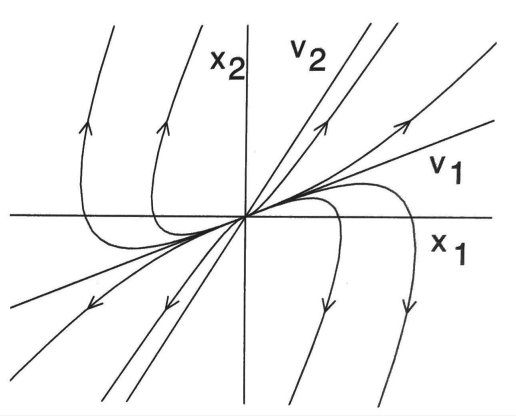
\includegraphics[height=3cm]{figures/un.png}
        \caption{Unstable node}
    \end{subfigure}
    \begin{subfigure}{0.3\textwidth}
        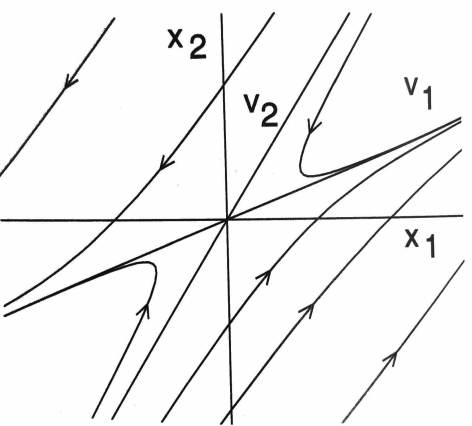
\includegraphics[height=3cm]{figures/sp.png}
        \caption{Saddle point}
    \end{subfigure}
    \label{fig:phase_portraits1}
\end{figure}

\begin{figure}[!htb]
    \centering
    \begin{subfigure}{0.3\textwidth}
        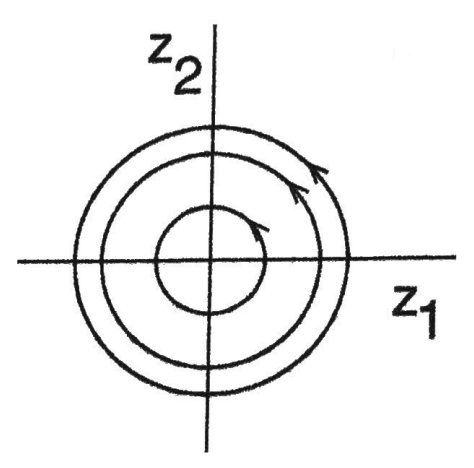
\includegraphics[height=3cm]{figures/cf.png}
        \caption{Center focus}
    \end{subfigure}
    \begin{subfigure}{0.3\textwidth}
        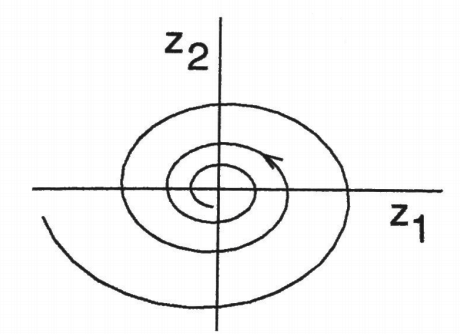
\includegraphics[height=3cm]{figures/sf.png}
        \caption{Stable focus}
    \end{subfigure}
    \begin{subfigure}{0.3\textwidth}
        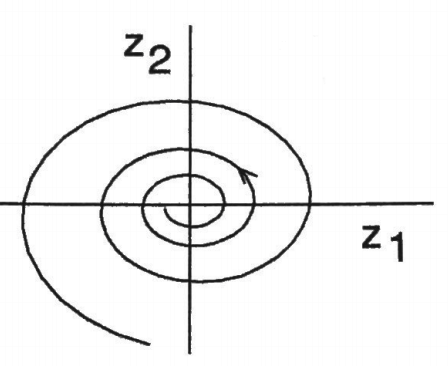
\includegraphics[height=3cm]{figures/uf.png}
        \caption{Unstable focus}
    \end{subfigure}
    \label{fig:phase_portraits2}
\end{figure}

\textbf{Topological equivalence:} if the real part of the eigenvalues are nonzero, then the local phase-portrait corresponds to the phase portrait of the linearized system.

\subsection{Periodic orbits and limit cycles}
\begin{definition}
    Periodic orbit: $\exists T>0$ s.t. $x(t+T)=x(t) \quad \forall t \geq 0$.
\end{definition}
\begin{definition}
    Limit cycle: non-trivial isolated periodic orbit.
\end{definition}

\begin{tcolorbox}[colback=white, colframe=teal]
\begin{lemma}
    Poincaré-Bendixson criterion:\\
    Let $M$ be a closed bounded subset of the plane s.t.
    \begin{itemize}[topsep=0pt]
        \item $M$ contains no $x^*$, or it
        contains only one $x^*$ with the property that
        the eigenvalues of the Jacobian matrix at $x^*$ have
        positive real parts (unstable focus or unstable node).
        \item Every trajectory starting in M stays in M $\forall t>t_0$.
    \end{itemize}
    Then $M$ contains a periodic orbit of the system.
\end{lemma}
\end{tcolorbox}

\begin{lemma}
    Bendixson negative criterion:\\
    If on a simply connected region $D$,$\frac{\partial f_{1}}{\partial x_{1}}+\frac{\partial f_{2}}{\partial x_{2}}$ is not identically zero and does not change sign, then the
    system has no periodic orbits lying entirely in $D$.
\end{lemma}

\begin{corollary}
    $C$ is a periodic orbit $\implies \Sigma_i I = 1$ (sum of indeces of equilibrium points in $C$, where saddle points have index -1 and others have index 1)
\end{corollary}

\section{Fundamental properties}
\begin{tcolorbox}[colback=white, colframe=teal]
\textbf{Lipschitz:} $\|f(t, x)-f(t, y)\| \leq L\|x-y\|$ \\
Either locally Lipschitz on $\mathbb{D}$ (L varies), Lipschitz in $\mathbb{D}$ or globally Lipschitz.
\end{tcolorbox}

\begin{theorem}
    Local existence and uniqueness:\\
    If
    \begin{itemize}[topsep=0pt]
        \item $f(t, x)$ is piecewise continuous in $t$,
        \item $f(t, x)$ is Lipschitz $\forall x, y \in B=\left\{x \in \mathbb{R}^{n} |\left\|x-x_{0}\right\| \leq r\right\} \forall t \in\left[t_{0}, t_{1}\right]$,
    \end{itemize}
    Then there exists a unique solution of the IVP $x(t)$
    on $t \in\left[t_{0}, t_{0}+\delta\right]$.
\end{theorem}

\section{Lyapunov stability}
\subsection{Stability of equilibrium points}
\textbf{Asymptotic stabilization problem:}
Find $\gamma(t, e)$ s.t. $e=0$ is an asymptotically stable equilibrium point.\\
Regulation vs. trajectory tracking.

\begin{definition}
    Stability: $x=0$ is stable iff
    $\forall \varepsilon>0 \quad \exists \delta(\varepsilon)>0 \quad \text { s.t. } \quad\|x(0)\|<\delta \Rightarrow\|x(t)\|<\varepsilon \quad \forall t \geq 0$
\end{definition}
\begin{definition}
    Asymptotic stability: $x = 0$ is (locally) asymptotically stable iff it is stable, and\\
    $\exists r>0 \quad \text { s.t. } \quad\|x(0)\|<r \Rightarrow \lim _{t \rightarrow \infty} x(t)=0$
\end{definition}
\begin{definition}
    Region of attraction: $B_{r}=\left\{x \in \mathbb{R}^{n}:\|x\|<r\right\}$. We denote $R_A$ as the union of all the regions of attraction.
\end{definition}
\begin{definition}
    Global asymptotic stability: $x = 0$ is GAS iff it is stable, and $\lim_{t \rightarrow \infty} x(t)=0 \quad \forall x(0)$
\end{definition}
\begin{definition}
    Exponential stability: $x = 0$ is exponentially stable iff\\
    $\exists r, k, \lambda>0$ s.t. $\|x(0)\|<r \Rightarrow\|x(t)\| \leq k\|x(0)\| e^{-\lambda t} \quad \forall t \geq 0$
\end{definition}
\begin{definition}
    Global exponential stability: $x = 0$ is GES iff
    $\exists k, \lambda>0$ s.t. $\forall x(0) \quad\|x(t)\| \leq k\|x(0)\| e^{-\lambda t} \quad \forall t \geq 0$
\end{definition}
\begin{remark}
    It is useful to think in terms of stability + convergence to seperate the different stability properties.
\end{remark}

\subsection{Lyapunov's indirect method}
\begin{tcolorbox}[colback=white, colframe=teal]
\begin{theorem}
    Lyapunov's indirect method:\\
    Let $x = 0$ be an equilibrium point for
    \begin{equation}
        \dot{x}=f(x), \quad f: \mathbb{D} \subset \mathbb{R}^{n} \rightarrow \mathbb{R}^{n} \quad \text { is } \quad C^{1}
    \end{equation}
    \begin{enumerate}[topsep=0pt]
        \item Linearize about $x=0, \dot{x} = Ax$, where $A=\left.\frac{\partial f}{\partial x}\right|_{x=0}$.
        \item Find the eigenvalues $\lambda_{1}(A), \ldots, \lambda_{n}(A)$.
        \item Categorize the eigenvalues:
        \begin{itemize}[topsep=0pt]
            \item $\forall i \quad \operatorname{Re}\left(\lambda_{i}\right)<0 \Rightarrow$ asymptotically(exponentially) stable
            \item $\exists i \quad \operatorname{Re}\left(\lambda_{i}\right)>0 \Rightarrow$ unstable
            \item $\forall i \quad \operatorname{Re}\left(\lambda_{i}\right)\leq 0 \Rightarrow$ inconclusive
        \end{itemize}
    \end{enumerate}
\end{theorem}
\end{tcolorbox}
While Lyapunov's indirect method is simple to use, the results are only local and often inconclusive. Let's see if we can do better ey?

\subsection{Lyapunov's direct method}
\begin{tcolorbox}[colback=white, colframe=teal]
\begin{definition}
    Lyapunov function:\\
    $V$ is a Lyapunov function for $x=0$ iff
    \begin{itemize}[topsep=0pt]
        \item $V$ is $C^1$
        \item $V(0)=0, \quad V(x)>0 \quad \text { in } \quad \mathbb{D} \backslash\{0\}$
        \item $\dot{V}(0)=0, \quad \dot{V}(x) \leq 0 \quad \text { in } \quad \mathbb{D} \backslash\{0\}$
    \end{itemize}
    If $\dot{V}(x) < 0 \quad \text { in } \quad \mathbb{D} \backslash\{0\}$ then $V$ is a strict Lyapunov function for $x=0$.
\end{definition}
\end{tcolorbox}

\begin{tcolorbox}[colback=white, colframe=teal]
\begin{theorem}
    Lyapunov's stability theorem:
    \begin{itemize}[topsep=0pt]
        \item If $\exists V(x)$ for $x=0$, then $x=0$ is stable.
        \item If $\exists$ strict $V(x)$ for $x=0$, then $x=0$ is asymptotically stable.
    \end{itemize}
\end{theorem}
\end{tcolorbox}

\begin{theorem}
    Chetaev's instability theorem:\\
    If $\dot{V}(x) > 0$ in a set $U = \{x \in B_r | V(x) > 0\}$, then $x=0$ is unstable.
\end{theorem}

\begin{tcolorbox}[colback=white, colframe=teal]
\begin{definition}
    \hl{Radially unboundedness:} $\quad \| x\| \rightarrow \infty \implies V(x) \rightarrow \infty$
\end{definition}
\end{tcolorbox}

\begin{theorem}
    If $\exists$ strict  $V : \mathbb{R}^n \rightarrow \mathbb{R}$ for $x=0$ and
    $V$ is radially unbounded,
    then $x=0$ is GAS.
\end{theorem}

\begin{theorem}
    If there exist a function $V : \mathbb{D} \rightarrow \mathbb{R}$ and constants $a, k_1, k_2, k_3 > 0$ s.t.
    \begin{itemize}[topsep=0pt]
        \item $V$ is $C^1$
        \item $k_{1}\|x\|^{a} \leq V(x) \leq k_{2}\|x\|^{a} \quad \forall x \in \mathbb{D}$
        \item $\dot{V}(x) \leq-k_{3}\|x\|^{a} \quad \forall x \in \mathbb{D}$
    \end{itemize}
    then $x=0$ is exponentially stable. If these conditions hold for $\mathbb{D} = \mathbb{R}^n$, then $x=0$ is GES. 
\end{theorem}

\begin{remark}
    $\lambda_{min}(P) \|x\|^2 \leq x^{\top} P x \leq \lambda_{max}(P) \|x\|^2$
\end{remark}

\begin{remark}
    How to deal with indeterminate signs in $\dot{V}$?
    \begin{itemize}[topsep=0pt]
        \item Completion of squares: $x_1 x_2 \leq \frac{1}{2}(x_1^2 + x_2^2)$
        \item Young's inequality: $x_1 x_2 \leq \epsilon x_1^2 + \frac{1}{4\epsilon}x_2^2$
        \item Cauchy-Schwarz' inequality: $\left|a_{1} x_{1}+a_{2} x_{2}+\cdots+a_{n} x_{n}\right| \leq \sqrt{\left(a_{1}^{2}+a_{2}^{2}+\cdots+a_{n}^{2}\right)}\|x\|_{2}$
    \end{itemize}
\end{remark}

\subsection{The invariance principle}
\begin{definition}
    Invariant set: $x(0) \in M \implies x(t) \in M \quad \forall t \in \mathbb{R}$
\end{definition}

\begin{definition}
    Positively invariant set: $x(0) \in M \implies x(t) \in M \quad \forall t \geq 0$
\end{definition}

\begin{definition}
    Level set: $\Omega_{c}=\left\{x \in \mathbb{R}^{n}: V(x) \leq c\right\}$
\end{definition}

\begin{remark}
    For $V(x)$ radially unbounded $\Omega_c$ is an invariant set.
\end{remark}

\begin{tcolorbox}[colback=white, colframe=teal]
\begin{theorem}
    La Salle's theorem:\\
    If $\exists V : \mathbb{D} \rightarrow \mathbb{R}$ s.t.
    \begin{itemize}[topsep=0pt]
        \item $V$ is $C^1$
        \item $\exists c>0 \text { such that } \Omega_{c}=\left\{x \in \mathbb{R}^{n} | V(x) \leq c\right\} \subset \mathbb{D} \text { is bounded }$
        \item $\dot{V}(x) \leq 0 \quad \forall x \in \Omega_{c}$
    \end{itemize}
    Let $E=\left\{x \in \Omega_{c} | \dot{V}(x)=0\right\}$. Let $M$ be the largest invariant set contained in $E$.
    Then $x(0) \in \Omega_{c} \Rightarrow x(t) \stackrel{t \rightarrow \infty}{\longrightarrow} M$.
\end{theorem}
\end{tcolorbox}

\begin{definition}
    \hl{Region of attraction:}\\
    Let $x=0$ be an asymptotically stable equilibrium point of the system $\dot{x} = f(x)$, where $f: \mathbb{D} \rightarrow \mathbb{R}^{n}$ is locally Lipschitz and $\mathbb{D} \subset \mathbb{R}^{n}$ contains the origin.
    Let $\phi\left(t, x_{0}\right)$ be the solution. Then the region of attraction is
    \begin{equation}
        R_{A}=\left\{x_{0} \in \mathbb{D} \quad | \quad \phi\left(t, x_{0}\right) \text { is defined } \forall t \geq 0 \text { and } \phi\left(t, x_{0}\right) \rightarrow 0 \text { as } t \rightarrow \infty\right\}
    \end{equation}
\end{definition}
(I.e. all the points with a corresponding solution that converges to the origin).
\begin{remark}
    GAS iff $R_A = \mathbb{R}^n$.
\end{remark}

\textbf{Estimate of $R_A$:} choose the largest set $\Omega_{c}$ in $\mathbb{D}$ which is bounded, and only the connected component of $\Omega_{c}$ that contains the origin.
Then this subset is a subset of $R_A$.

\subsection{Stability analysis of time-variant systems}
We now consider the system $\dot{x} = f(t, x)$.

\begin{definition}
    Stability: $\forall \varepsilon>0, \quad \exists \delta\left(\varepsilon, t_{0}\right)>0 \quad \text{s.t.} \quad \left\|x\left(t_{0}\right)\right\|<\delta \Rightarrow\|x(t)\|<\varepsilon \quad \forall t \geq t_{0} \geq 0$
\end{definition}
\begin{definition}
    Uniform stability: stable with $\delta\left(\varepsilon, t_{0}\right) = \delta\left(\varepsilon\right)$.
\end{definition}
\begin{definition}
    Asymptotic stability: stable and $\exists c\left(t_{0}\right)>0 \quad \text {s.t.} \quad \left\|x\left(t_{0}\right)\right\|<c \Rightarrow x(t) \stackrel{t \rightarrow \infty}{\longrightarrow} 0$.
\end{definition}
\begin{definition}
    Uniform asymptotic stability: asymptotically stable with $\delta\left(\varepsilon, t_{0}\right) = \delta\left(\varepsilon\right)$.
\end{definition}
\begin{definition}
    Global uniform asymptotic stability: uniform stability with $\delta(\varepsilon) \stackrel{\varepsilon \rightarrow \infty}{\longrightarrow} \infty$ and $\forall c>0 \quad\left\|x\left(t_{0}\right)\right\|<c \Rightarrow x(t) \stackrel{t \rightarrow \infty}{\longrightarrow} 0$ uniformly in $t_0$.
\end{definition}
\begin{definition}
    Exponential stability: $\exists c, k, \lambda>0 \quad \text { s.t. } \quad\|x(t)\| \leq k\left\|x\left(t_{0}\right)\right\| e^{-\lambda\left(t-t_{0}\right)} t \geq t_{0} \geq 0 \left\|x\left(t_{0}\right)\right\| \leq c$.
    GES if $\forall c$.
\end{definition}

\begin{definition}
    A continuous function $\alpha:[0, a) \rightarrow[0, \infty)$ is a \hl{class $\mathscr{K}$ function} iff:\\
    $\alpha(0)=0$ and $\alpha(r)$ is strictly increasing, i.e. $\frac{\partial \alpha}{\partial r}>0 \quad \forall r>0$.
\end{definition}
\begin{definition}
    If in addition $a \rightarrow \infty$ and $\alpha(r) \rightarrow \infty \text { as } r \rightarrow \infty$, then $\alpha$ is a \hl{class $\mathscr{K}_\infty$ function.}
\end{definition}
\begin{definition}
    A continuous function $\beta:[0, a) \times[0, \infty) \rightarrow[0, \infty)$
    is a \hl{class $\mathscr{KL}$ function} if for each fixed $s$
    \begin{itemize}[topsep=0pt]
        \item $\beta(r,s)$ is a class $\mathscr{K}$ function w.r.t. $r$
    \end{itemize}
    and for each fixed $r$
    \begin{itemize}[topsep=0pt]
        \item $\beta(r,s)$ is decreasing w.r.t. $s$,
        \item $\beta(r,s) \rightarrow 0$ as $s \rightarrow \infty$.
    \end{itemize}
\end{definition}

We can now define stability in terms of class $\mathscr{K}$ functions:
\begin{definition}
    Uniform stability: $\exists$ class $\mathscr{K}$ function $\alpha$ and $\exists c > 0$ s.t.
    $\|x(t)\| \leq \alpha\left(\left\|x\left(t_{0}\right)\right\|\right) \forall t \geq t_{0} \geq 0, \quad \forall\left\|x\left(t_{0}\right)\right\|<c$.
\end{definition}
\begin{definition}
    Uniform asymptotic stability: $\exists$ class $\mathscr{KL}$ function $\beta$ and $\exists c > 0$ s.t.
    $\|x(t)\| \leq \beta\left(\left\|x\left(t_{0}\right)\right\|, t-t_{0}\right) \forall t \geq t_{0} \geq 0, \quad \forall\left\|x\left(t_{0}\right)\right\|<c$.
    GUAS if $\forall c$.
\end{definition}

\begin{definition}
    $V(t,x)$ is \hl{positive definite} iff
    \begin{itemize}[topsep=0pt]
        \item $V(t,0)=0$
        \item $V(t,x) \geq W_1(x)$
    \end{itemize}
    $\forall t \geq 0, W_1(x)>0$
\end{definition}
\begin{definition}
    $V(t,x)$ is \hl{decrescent} iff
    \begin{itemize}[topsep=0pt]
        \item $V(t,0)=0$
        \item $V(t,x) \leq W_2(x)$
    \end{itemize}
    $\forall t \geq 0, W_2(x)>0$
\end{definition}

We can summarize the stability theorems for time-varying systems like this:
\begin{center}
    \begin{tabular}{|c|c|c|c|c|}
        \hline
        & Stable & Uniformly stable & UAS & GUAS \\
        \hline
        $V$ & Pos. def. & Pos. def., decrescent & Pos. def., decrescent. & Pos. def., decrescent, radially unbounded \\
        \hline
        $\dot{V}$ & Neg. semidef. & Neg. semidef. & Neg. def. & Neg. def. \\
        \hline
        & $\forall x \in \mathbb{D}$ & $\forall x \in \mathbb{D}$ & $\forall x \in \mathbb{D}$ & $\forall x \in \mathbb{R}^n$ \\
        \hline
    \end{tabular} 
    \label{tab:stability}
\end{center}

\textbf{Estimate of $R_A$:} $B_{r}=\left\{x \in \mathbb{R}^{n}:\|x\| \leq r\right\} \subset \mathbb{D}, c<\min _{\|x\|=r} W_{1}(x) \implies \left\{x \in B_{r}: W_{2}(x) \leq c\right\}$ is a region of attraction, when the origin is UAS.

\begin{tcolorbox}[colback=white, colframe=teal]
\begin{lemma}
    Barbalat's lemma: \\
    Let $\dot{f} : \mathbb{R} \rightarrow \mathbb{R}$ be uniformly continuous on $[0, \infty)$. If $\lim _{t \rightarrow \infty} f(t)$ exists and is finite, then $\dot{f} \rightarrow 0 \text { as } t \rightarrow \infty$.\\
    Rephrased: if $V$ is lower bounded, $\dot{V} \leq 0$ and $\ddot{V}$ is uniformly bounded, then $\dot{V} \rightarrow 0$ as $t \rightarrow \infty$.
\end{lemma}
\end{tcolorbox}

\section{Input-to-state stability}
\subsection{Input-to-state stability}
Now we consider the system $\Sigma: \dot{x}=f(t, x, u)$, where we consider $u(t)$ to be a disturbance/modelling error.

\begin{definition}
    \hl{Input-to-state stability (ISS):} $\exists \beta \in \mathscr{K} \mathscr{L}, \gamma \in \mathscr{K} \text { s.t. } \left\|x\left(t, x_{0}, u\right)\right\| \leq \max \left\{\beta\left(\left\|x\left(t_{0}\right)\right\|, t-t_{0}\right), \gamma\left(\|u\|_{\infty}\right)\right\}$
\end{definition}
\begin{remark}
    This is really just an extension of GUAS that says that $x$ is bounded the input as well. So naturally if $\Sigma$ is ISS then it is also 0-GUAS.
\end{remark}

\begin{tcolorbox}[colback=white, colframe=teal]
\begin{definition}
    $V:[0, \infty) \times \mathbb{R}^{n} \rightarrow \mathbb{R}$ is an \hl{ISS-LF} for $\Sigma \text { iff }$
    \begin{itemize}[topsep=0pt]
        \item $V$ is $C^1$.
    \end{itemize}
    $\exists \alpha_{1}, \alpha_{2} \in \mathscr{K}_{\infty} \text { and } \rho \in \mathscr{K} \text { s.t. }$
    \begin{itemize}[topsep=0pt]
        \item $\alpha_{1}(\|x\|) \leq V(t, x) \leq \alpha_{2}(\|x\|)$
        \item $\dot{V}(t, x)=\frac{\partial V}{\partial x} f+\frac{\partial V}{\partial t} \leq-W_{3}(x) \quad\ \forall \|x\| \geq \rho(\|u\|)>0$
    \end{itemize}
    where $W_3 > 0$.\\
    It can be shown that $\gamma=\alpha_{1}^{-1} \circ \alpha_{2} \circ \rho$.\\
    $\exists \mathrm{ISS}-\mathrm{LF} \text { for } \Sigma \Rightarrow \Sigma \text { is } \mathrm{ISS}$
\end{definition}
\end{tcolorbox}

\begin{lemma}
    if $f \text { is } C^{1} \text { and globally Lipschitz in }(x, u)$, then
    $\Sigma \text { is } 0-\mathrm{GES} \Rightarrow \Sigma \text { is } \mathrm{ISS}$
\end{lemma}

\begin{theorem}
    Consider the cascaded system $\Sigma_{2} \longrightarrow \Sigma_{1}$, where $\Sigma_{1}: \dot{x}_{1}=f_{1}\left(t, x_{1}, x_{2}\right)$ and $\Sigma_{2}: \dot{x}_{2}=f_{2}\left(t, x_{2}\right)$.\\
    If $\Sigma_2$ is GUAS and $\Sigma_1$ is ISS, then the cascaded system is GUAS. 
\end{theorem}

\subsection{Input-output stability}
We consider the system $y=H u$.
\begin{definition}
    $\mathscr{L}_{p}^{m}$ space:
    $\quad u \in \mathscr{L}_{p}^{m} \quad 1 \leq p<\infty \quad \Leftrightarrow \quad\|u\|_{\mathscr{L}_{p}}=\left(\int_{0}^{\infty}\|u(t)\|_{\bar{p}}^{p} d t\right)^{\frac{1}{p}}<\infty$
\end{definition}
\begin{remark}
    This makes $\mathscr{L}_{2}$ the space of all continuous, square-integrable functions, for instance.
\end{remark}
\begin{definition}
    $\mathscr{L}_{pe}^{m}$ space:
    $u \in \mathscr{L}_{p e}^{m} \Leftrightarrow u_{\tau} \in \mathscr{L}_{p}^{m} \quad \forall \tau \in[0, \infty)$, where $u_\tau$ is the truncated version if $u$.
\end{definition}

\begin{tcolorbox}[colback=white, colframe=teal]
\begin{definition}
    $H: \mathscr{L}_{p e}^{m} \rightarrow \mathscr{L}_{p e}^{q} \text { is }$ \hl{$\mathscr{L}_{p}$ stable} iff
    \begin{itemize}[topsep=0pt]
        \item $\exists \alpha \text { class } \mathscr{K} \quad \alpha:[0, \infty) \rightarrow[0, \infty)$
        \item $\exists \text { constant } \beta \geq 0$
    \end{itemize}
    s.t. $\left\|(H u)_{\tau}\right\|_{\mathscr{L}_{p}} \leq \alpha\left(\left\|u_{\tau}\right\|_{\mathscr{L}_{p}}\right)+\beta \quad \forall u \in \mathscr{L}_{p e}^{m} \text { and } \tau \in[0, \infty)$
\end{definition}
\end{tcolorbox}

\begin{definition}
    \hl{Finite-gain $\mathscr{L}_{p}$ stable:}
    $\exists\gamma, \beta \geq 0$ s.t. $\left\|(H u)_{\tau}\right\|_{\mathscr{L}_{p}} \leq \gamma\left\|u_{\tau}\right\|_{\mathscr{L}_{p}}+\beta$
\end{definition}
\begin{definition}
    Causal system: $(H u)_{\tau}=\left(H u_{\tau}\right)_{\tau}$\\
    The two definitons above hold for non-truncated signals if the systems are causal.
\end{definition}

\begin{theorem}
    Small-gain theorem:\\
    The feedback interconnection of $H_1$ and $H_2$ are finite-gain $\mathscr{L}_{p}$ stable
    iff $\gamma_1 \gamma_2 < 1$.
\end{theorem}
\begin{figure}[!htb]
        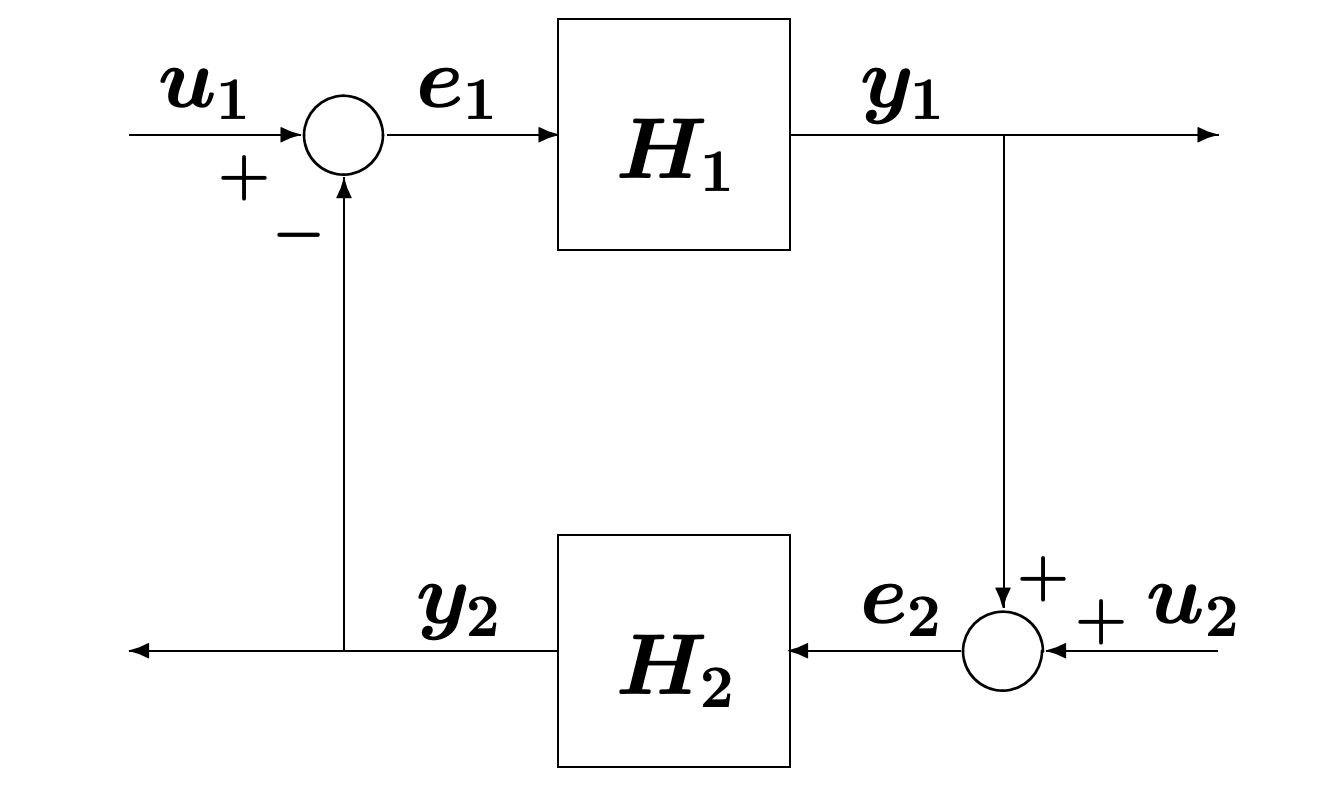
\includegraphics[width = 0.6\textwidth]{figures/fb.png}
        \caption{Feedback interconnection}
\end{figure}
\newpage
\section{Passivity}
\subsection{Passivity for memoryless functions}
Consider the memoryless function $y=h(t, u) \quad h:[0, \infty) \times \mathbb{R}^{p} \rightarrow \mathbb{R}^{p}$.
\begin{definition}
    The system is \hl{passive} if $u^{\top} y \geq 0$ and lossless if $u^{\top} y=0$.\\
    The system is \hl{input-strictly passive} if $u^{\top} y \geq u^{\top} \varphi(u)$, where $u^{\top} \varphi(u)>0 \quad \forall u \neq 0$.\\
    The system is \hl{output-strictly passive} if $u^{\top} y \geq y^{\top} \rho(y)$, where $y^{\top} \rho(y)>0 \quad \forall y \neq 0$.
\end{definition}

\subsection{Passivity for dynamical systems}
Now we extend this property for dynamical systems: $\Sigma: \quad \dot{x}=f(x, u), y=h(x, u)$\\
where $f: \mathbb{R}^{n} \times \mathbb{R}^{p} \rightarrow \mathbb{R}^{n}$ is locally Lipschitz and $h: \mathbb{R}^{n} \times \mathbb{R}^{p} \rightarrow \mathbb{R}^{p}$ is continuous, and $f(0,0)=0 \text { and } h(0,0)=0$.

\begin{tcolorbox}[colback=white, colframe=teal]
\begin{definition}
    The system $\Sigma$ is \hl{passive} iff
    $u^{\top} y \geq \dot{V} \quad \forall(x, u) \in \mathbb{R}^{n} \times \mathbb{R}^{p}$\\
    The system is \hl{lossless} if  $u^{\top}y = \dot{V}$.\\
    The system is \hl{input-strictly passive} if $u^{T} y \geq \dot{V}+u^{T} \varphi(u), \quad u^{T} \varphi(u)>0 \quad \forall u \neq 0$.\\
    The system is \hl{output-strictly passive} if $u^{T} y \geq \dot{V}+y^{T} \rho(y), \quad y^{T} \rho(y)>0 \quad \forall y \neq 0$.\\
    The system is \hl{(state-) strictly passive} if $u^{T} y \geq \dot{V}+\psi(x), \quad \psi(x)>0$.
\end{definition}
\end{tcolorbox}

\begin{remark}
    Passivity really just generalizes the idea that the change of stored energy in the system should be less than the energy supplied to the system.
\end{remark}

\subsection{Passivity and Lyapunov stability}
\begin{lemma}
    If $\Sigma$ is passive with a positive definite $V(x)$, then the origin of $\dot{x}=f(x, 0)$ is stable.
\end{lemma}
\begin{lemma}
    If $\Sigma$ is output-strictly passive with $\rho(y) = \delta y, \delta < 0$, then $\Sigma$ is finite-gain $\mathscr{L}_{2}$ stable with $\gamma \leq \frac{1}{\delta}$.
\end{lemma}

\begin{definition}
    Zero state observability: no solution of $\dot{x}=f(x, 0)$ can stay identically in $S=\left\{x \in \mathbb{R}^{n} | h(x, 0)=0\right\}$ other than the trivial solution $x(t)=0$.
\end{definition}
\begin{lemma}
    The origin of $\dot{x}=f(x, 0)$ is asymptotically stable if $\Sigma$ is state-strictly passive, or output-strictly passive and zero state observable.
    If $V(x)$ is radially unbounded $\dot{x}=f(x, 0)$ is GAS.
\end{lemma}

\begin{theorem}
    If $H_1$ and $H_2$ is passive, then the feedback interconnection of $H_1$ and $H_2$ is passive with $V=V_1+V_2$.
\end{theorem}
\begin{theorem}
    If $H_1$ and $H_2$ satisfies $e_{i}^{T} y_{i} \geq \dot{V}_{i}+\varepsilon_{i} e_{i}^{T} e_{i}+\delta_{i} y_{i}^{T} y_{i} i=1,2$ and $\varepsilon_{1}+\delta_{2}>0, \varepsilon_{2}+\delta_{1}>0$, \\
    then $\Sigma$ is finite-gain $\mathscr{L}_{2}$ stable.
\end{theorem}
\begin{theorem}
    If $H_1$ and $H_2$ are state-strictly passive,\\
    or $H_1$ and $H_2$ are output-strictly passive and zero state observable,\\
    or $H_1$ is state-strictly passive and $H_2$ is output-strictly passive and zero state observable or opposite,\\
    then $\Sigma$ is 0-AS. If $V_1$ and $V_2$ are radially unbounded then $\Sigma$ is 0-GAS.
\end{theorem}

\section{Nonlinear control}
\subsection{Lyapunov control design}
\begin{tcolorbox}[colback=white, colframe=teal]
\begin{itemize}[topsep=0pt]
    \item Propose a LFC $V(t,x)$, typically as desired energy in system.
    \item Choose $u=g(t,x)$ s.t. $\dot{V}<0$ or $\dot{V}\leq0$ with La Salle / Barbalat.
\end{itemize}
\end{tcolorbox}

\subsection{Passivity-based control}

\begin{tcolorbox}[colback=white, colframe=teal]
\begin{theorem}
    For the LTI system $y(s)=h(s)u(s)$ with $\operatorname{Re}\left(p_{i}\right)<0, \forall i$ we have:
    \begin{itemize}[topsep=0pt]
        \item Passivity $\Leftrightarrow \operatorname{Re}[h(j \omega)] \geq 0 \forall \omega$ (note that if $h(s)$ has an integrator as well and $\operatorname{Re}\left(z_{i}\right)<0$ this still holds)
        \item Input-strict passivity $\Leftrightarrow \operatorname{Re}[h(j \omega)] \geq \delta>0 \forall \omega$, with $\varphi(u)=\delta u$
        \item Output-strict passivity $\Leftrightarrow \exists \varepsilon>0 \text { s.t. } \operatorname{Re}[h(j \omega)] \geq \varepsilon|h(j \omega)|^{2} \forall \omega$, with $\rho(y)=\varepsilon y$
    \end{itemize}
\end{theorem}
\end{tcolorbox}
\begin{remark}
    This says that with non-negative real part the system is passive, with a strictly positive real part it is input-strictly passive and if it  is lower bounded by the square of the magnitude it is output-strictly passive.
\end{remark}

\begin{remark}
    Note that the previously discussed passivity theorems can be applied for passivity-based control. \\
    Notably that means that if the controller and plant are passive, then the closed-loop system is passive.\\
    Also if the controller is input- and output strictly passive and the plant is passive, then the system is finite gain $\mathscr{L}_2$ stable.
    The final passivity theorem can naturally also be applied.
\end{remark}

\begin{tcolorbox}[colback=white, colframe=teal]
\begin{theorem}
    Consider $H_{1}$ with $\dot{x}=f(x, u)$ locally Lipschitz and $y = h(x)$ continuous, both zero in the origin.\\
     Also consider $H_2 :\phi(y)$ locally Lipschitz, memoryless and zero in origin.\\
     If $H_1$ is passive with $V>0$, radially unbounded and zero state observable, and $H_2$ satisifes $y^{\top} \phi(y) > 0, y \neq 0$ (passive, but not lossness) then the origin is GAS.
\end{theorem}
\end{tcolorbox}

\textbf{Choice of y:} for $\dot{x}=f(x)+G(x) u$, if $\exists$ LF $V(x)$ radially unbounded, let $y=\left[\frac{\partial V}{\partial x} G(x)\right]^{T}$ for the system to be passive.
\hl{\textbf{Feedback} \textbf{passivation:}} choose $u=\alpha(x)+\beta(x) v, y=h(x)$ s.t. $\dot{x}=f(x)+G(x) u$ has desired passivity properties $v \mapsto y$.

\subsection{Feedback linearization}
\subsubsection{Input-state linearization}
Consider $\dot{x}=f(x)+G(x) u$. Find a state transformation $z=T(x)$ and input transformation $u = \alpha(x) + \beta(x)v$ s.t. the new system in $z$ coordinates is linear and controllable.
This is rearily possible to do, so we consider input-output linearization instead:

\subsubsection{Input-output linearization}
We now consider the system $\begin{array}{l}{\dot{x}=f(x)+g(x) u} \\ {y=h(x)}\end{array}$.
\begin{definition}
    \hl{Lie derivative:} $L_{f} h=\frac{\partial h}{\partial x} f, \quad L_{f}^{2} h=\frac{\partial L_{f} h}{\partial x} f, \quad \dots \quad L_{f}^{i} h=L_{f}\left(L_{f}^{i-1} h\right)$
\end{definition}
\begin{definition}
    The system has \hl{relative degree $\rho$} $ \text { in a region } \mathbb{D}_{0} \subset \mathbb{D} \subset \mathbb{R}^{n} \text { if }$
    \begin{equation}
    \left.\begin{array}{l}{L_{g} L_{f}^{i-1} h=0, \quad 1 \leq i \leq \rho-1} \\ {L_{g} L_{f}^{\rho-1} h \neq 0}\end{array}\right\} \forall x \in \mathbb{D}_{0}
    \end{equation}
\end{definition}
\begin{remark}
    (the number of differentiations of $y$ before $u$ appears)
\end{remark}
\begin{remark}
    For linear systems we have $\rho = n-m$.
\end{remark}
\begin{remark}
    If the relative degree is well defined in the region of interest $\mathbb{D}$, then the system can be input-output linearized.
\end{remark}

\begin{definition}
   \hl{Zero dynamics:} internal dynamics when output is kept at zero by the input i.e. $\psi = 0, \dot{\phi} = f_o(\phi, 0)$.
\end{definition}
\begin{definition}
    \hl{Minimum-phase system:} the zero-dynamics are asymptotically stable.
\end{definition}

\begin{tcolorbox}[colback=white, colframe=teal]
    \textbf{Input-output linearization:}
    \begin{enumerate}
        \item \textbf{Find the relative degree $\rho$}
        \item \textbf{Write the system in normal form}\\
        Let $\psi_1 = y, \psi_2 = \dot{y}, \dots$
        The \hl{external dynamics} are then $\dot{\psi_1} = \psi_2, \dots, \dot{\psi}_{\rho}=L_{f}^{\rho} h+L_{g} L_{f}^{\rho-1} h \cdot u$.\\
        Let $\phi_1, \dots, \phi_{n-\rho}$ and $z = T(x) =
        [\begin{array}{cc}\varphi^{\top} & \psi^{\top} \end{array}]^{\top}$.\\
        Choose $\varphi$ s.t. $T$ is a diffeomorphism, $L_{g} \varphi_{i}=0$ and $\varphi_i(0)=0$.\\
        If the Jacobian $\left.\frac{\partial T}{\partial x}\right|_{x_{0}}$ is nonsingular, then $T$ is a diffeomorphism. Then the \hl{internal dynamics} are $\dot{\psi} = \dots$.
        We can then finally write the system in \hl{normal form:} $\dot{z} = \dots$.
        \item \textbf{Choose u to cancel nonlinearities}
        \begin{equation}
            u=\frac{1}{L_{g} L_{f}^{\rho-1} h}\left(-L_{f}^{\rho} h+v\right) \quad \implies \quad \psi_{\rho} = v
        \end{equation}
        \item \textbf{Analyze the zero-dynamics}
        \item \textbf{Choose $v$ to solve the control problem}\\
        This is a special case of the system $\dot{\varphi}=f_{0}(\varphi, \psi), \quad \dot{\psi}=A \psi+B v$.
        \begin{lemma}
            If the system is minimum phase and $v=-K\psi$ is chosen s.t. $(A-BK)$ is Hurwitz, then the origin of the system is asymptotically stable.
        \end{lemma}
        \begin{lemma}
            If $\dot{\phi} = f_0(\phi, \psi)$ is ISS, then the system is GAS.
        \end{lemma}
        For tracking we have $v=-K e+y_{d}^{(\rho)}$, but the same results apply, expect $\phi$ is now only bounded.
    \end{enumerate}
\end{tcolorbox}

\subsection{Adaptive control}
\subsubsection{MRAC for SISO systems}
Consider the SISO system $\dot{x} = a_p x + c_p f(x) + b_p u$.
\begin{tcolorbox}[colback=white, colframe=teal]
    \textbf{SISO MRAC:}
    \begin{enumerate}
    \item \textbf{Specify desired closed-loop behaviour} by reference model:
        $\dot{x}_m = a_m x_m + b_m r(t)$
    \item \textbf{Choose control law} s.t. plant output tracks reference model output when parameters are exactly known, by deriving error dynamics. Then replace parameters by estimates. 
    \item \textbf{Choose adaptation law} ($\dot{\hat{a}}_x, \dot{\hat{a}}_f, \dot{\hat{a}}_r$) by first deriving new tracking error dynamics in terms of estimation errors, and then choosing adaptation law from suitable Lyapunov function e.g.
    \begin{equation}
        V(e, \tilde{a}) = \frac{1}{2}e^2 + \frac{|b_p|}{2\gamma_x}\tilde{a}_x^2 +\frac{|b_p|}{2\gamma_f}\tilde{a}_f^2 +\frac{|b_p|}{2\gamma_r}\tilde{a}_r^2
    \end{equation}
    By letting
    \begin{equation}
        \dot{\hat{a}}_x = - \gamma_x \text{sgn}(b_p)ex, \quad \dot{\hat{a}}_f = - \gamma_f \text{sgn}(b_p)ef, \quad \dot{\hat{a}}_r = - \gamma_r \text{sgn}(b_p)er
    \end{equation}
    the error will go to zero by Barbalat's lemma.
\end{enumerate}
\end{tcolorbox}

\begin{figure}[!htb]
    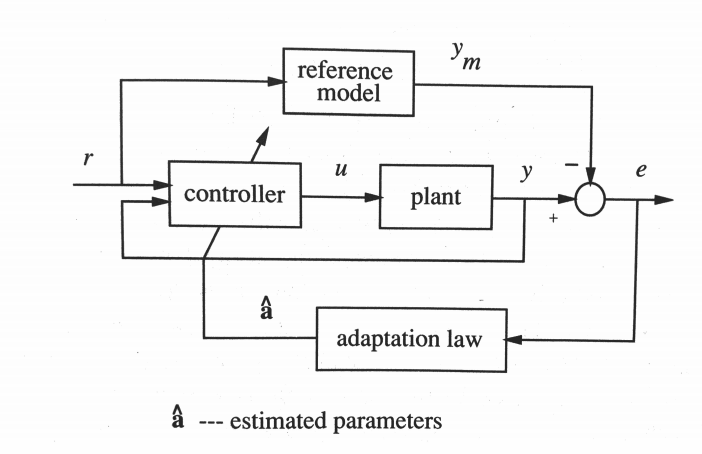
\includegraphics[width = 0.6\textwidth]{figures/mrac.png}
    \caption{Model reference adaptive control loop}
\end{figure}

\subsubsection{Adaptive tracking control for a class of MIMO systems}
Consider the system $M(q) \ddot{q}+C(q, \dot{q}) \dot{q}+D(q) \dot{q}+g(q)=u$, with $M>0, \dot{M}-2 C \text { is skew symmetric, } z^{T} D z>0 \quad \forall z \neq 0$.\\
While the system is nonlinear it is linear in the unknown parameters $a$ by the Regression matrix $Y$:
\begin{equation}
    M(q) \ddot{q}+C(q, \dot{q}) \dot{q}+D(q) \dot{q}+g(q)=Y(q, \dot{q}, \ddot{q}) a
\end{equation} 

\begin{tcolorbox}[colback=white, colframe=teal]
    \textbf{Adaptive MIMO tracking control:}
    \begin{enumerate}
        \item Given the desired trajectory $q_d(t), \dot{q}_d(t), \ddot{q}_d(t)$ bounded.
        \item \textbf{Choose control law:}\\
        We introduce the virtual reference velocity $s= \dot{e} + \lambda e = \dot{q} - \dot{q}_r$, where $\dot{q}_{r}=\dot{q}_{d}
        -\Lambda\left(q-q_{d}\right)$.\\
        \begin{equation}
            u=\hat{M}(q) \ddot{q}_{r}+\hat{C}(q, \dot{q}) \dot{q}_{r}+\hat{D}(q) \dot{q}_{r}+\hat{g}(q)-K_{p}\left(q-q_{d}\right)-K_{d}\left(\dot{q}-\dot{q}_{d}\right) = Y\left(q, \dot{q}, \dot{q}_{r}, \ddot{q}_{r}\right) \hat{a}-K_{p} e-K_{d} \dot{e}
        \end{equation}
        From $V(s)= \frac{1}{2} s^{\top}Ms$ and the cascade stability theorem we get GUAS with perfect tracking.
        \item \textbf{Choose an adaptation law} such that tracking is achieved asymptotically. Again done by deriving error dynamics and analyzing Lyapunov function with Barbalat's lemma:
        \begin{equation}
            V(s, \tilde{a}) = \frac{1}{2} s^{\top}Ms + \frac{1}{2} \tilde{a}^{\top}\Gamma^{-1}\tilde{a} \implies \dot{\tilde{a}} = - \Gamma Y^{\top}s
        \end{equation}
        
    \end{enumerate}
\end{tcolorbox}

\subsection{Backstepping}
We consider the system
\begin{equation}
\left[\begin{array}{c}{\dot{x}_{1}} \\ {\dot{x}_{2}} \\ {\vdots} \\ {\dot{x}_{n}}\end{array}\right]=f\left(\left[\begin{array}{c}{x_{1}} \\ {x_{2}} \\ {\vdots} \\ {x_{n}}\end{array}\right]+g\left(\left[\begin{array}{c}{x_{1}} \\ {x_{2}} \\ {\vdots} \\ {x_{n}}\end{array}\right]\right) \cdot x_{n+1}\right., \quad
    \dot{x}_{n+1}=u
\end{equation}
Which we can identify as the cascaded system ${\Sigma_{1}:} {\dot{\eta}=f(\eta)+g(\eta) \xi}, \quad {\Sigma_{2}:} {\dot{\xi}=u}$. \\ We can regard $\xi$ as the virtual control input of $\Sigma_1$.

\begin{tcolorbox}[colback=white, colframe=teal]
    \textbf{Integrator backstepping:}
    \begin{enumerate}
        \item \textbf{Find stabilizing function for $\Sigma_1$}\\
        $\xi=\varphi(\eta), \quad \varphi(0)=0$ s.t. $\xi = 0$ is asymptotically stable by some $V_1(\eta)$.
        \item \textbf{Design actual control input $u$}
        \begin{enumerate}
            \item Introduce error variable $z=\xi-\varphi(\eta)$.
            \item Derive dynamics in $(\eta, z)$ coordinates.
            \item Choose LFC $V_2(\eta, z) = V_1(\eta) + \frac{1}{2}x^2$.
            \item Find $u$ that asymptotically stabilizes $(\eta, z) = (0,0)$. Generally we get:
            \begin{equation}
                u=-\frac{\partial V}{\partial \eta} g(\eta)+\dot{\varphi}-k z
            \end{equation}
            If $V_2$ is radially unbounded in $\eta$ and $\mathbb{D} = \mathbb{R}^n$ the results are global.
        \end{enumerate}
    \end{enumerate}
\end{tcolorbox}
\begin{remark}
    Note that this is a recursive process, and you may therefore do several steps of finding virtual control inputs before finally finding $u$. Also note that the method works fine even if $\Sigma_2$ is more exotic.
\end{remark}
